\chapter{Frontend Implementation}
\label{ch:frontend}

This chapter describes the frontend implementation, focusing on the key architectural decisions rather than implementation details.

\section{Console UI Architecture}

The Next.js console (\texttt{frontend/app/console/page.tsx}) provides a real-time interface for voice agent interaction. The console is designed as a single-page application with the following components:

\textbf{Key Components:}
\begin{itemize}
    \item \textbf{Control Deck}: Record/stop buttons with keyboard shortcuts
    \item \textbf{Status Indicators}: Real-time ASR model loading and readiness state
    \item \textbf{Waveform Visualizer}: Audio level visualization using Web Audio API's AnalyserNode
    \item \textbf{Transcript Terminal}: Timestamped display of partial and final transcriptions
    \item \textbf{Widget Area}: Dynamic rendering of price estimates and property listings
    \item \textbf{Agent Reply Panel}: Streaming display of LLM-generated responses
\end{itemize}

\begin{figure}[!htbp]
\centering
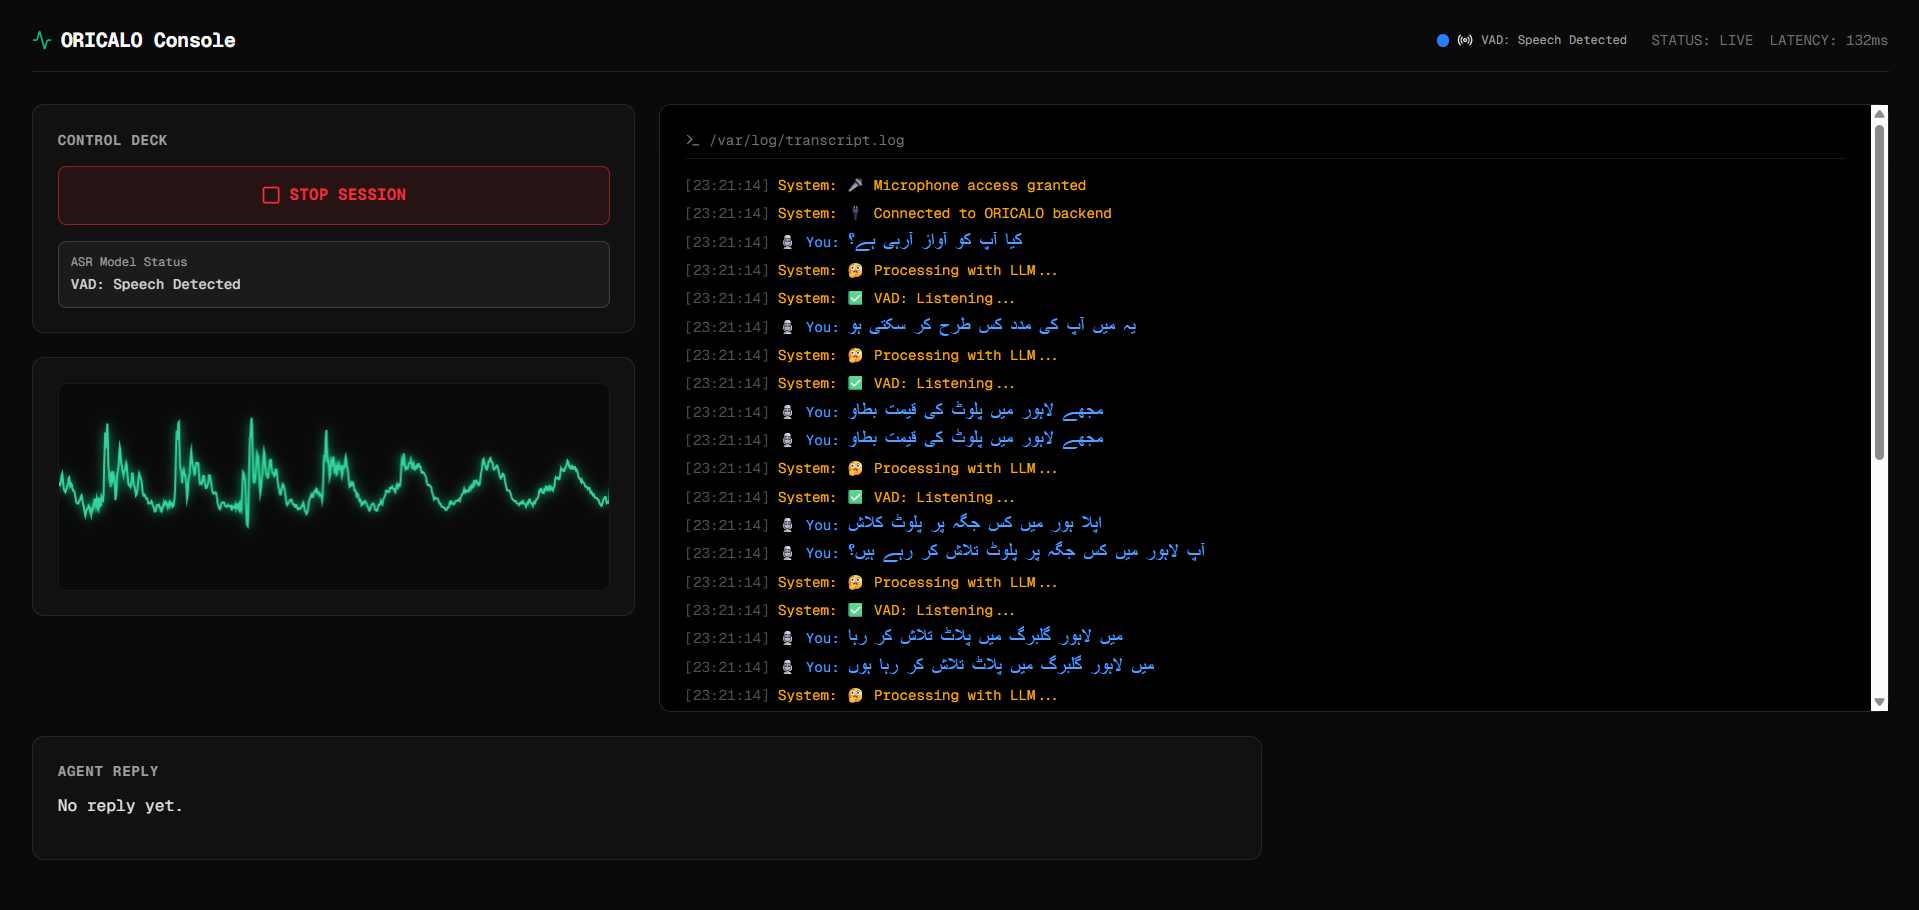
\includegraphics[width=0.95\textwidth]{ThesisFigs/UI_screenshot}
\caption{ORICALO Console Interface showing the transcript terminal, waveform visualizer, and control deck}
\label{fig:console-ui}
\end{figure}

\section{Audio Streaming Architecture}

The frontend uses Web Audio API for raw PCM streaming instead of MediaRecorder. This architectural choice provides several advantages:

\begin{itemize}
    \item \textbf{Lower Latency}: Direct access to audio samples without codec overhead
    \item \textbf{Fixed Sample Rate}: Consistent 16kHz sampling required by Whisper ASR
    \item \textbf{Real-time Processing}: ScriptProcessor nodes enable per-buffer operations
\end{itemize}

The audio pipeline converts Float32 samples to Int16 PCM format, base64 encodes the buffer, and transmits via WebSocket in 4096-sample chunks (156ms at 16kHz).

\section{Widget System}

The UI implements dynamic widgets triggered by action payloads from the dialogue API:

\begin{table}[!htbp]
\centering
\caption{Frontend Widget Components}
\label{tab:widgets}
\begin{tabular}{|l|l|p{6cm}|}
\hline
\textbf{Component} & \textbf{File} & \textbf{Purpose} \\ \hline
PriceWidget & \texttt{PriceWidget.tsx} & Display price range with confidence indicator \\ \hline
RagWidget & \texttt{RagWidget.tsx} & Grid of property listing cards with key details \\ \hline
WaveformVisualizer & \texttt{WaveformVisualizer.tsx} & Real-time audio waveform using canvas \\ \hline
\end{tabular}
\end{table}

Each widget is designed for voice-first interaction, with:
\begin{itemize}
    \item High-contrast colors for quick visual scanning
    \item Large typography for readability
    \item Minimal interaction requirements (information display focused)
    \item Smooth animations for state transitions
\end{itemize}

\section{WebSocket Communication}

The frontend maintains a persistent WebSocket connection to the backend for:

\begin{itemize}
    \item \textbf{Audio Upload}: Streaming PCM audio chunks for ASR processing
    \item \textbf{Transcript Events}: Receiving partial and final transcriptions
    \item \textbf{Status Updates}: Model loading states and error notifications
\end{itemize}

A separate HTTP endpoint handles dialogue API calls with NDJSON streaming for token-by-token response display.

\section{Implementation Summary}

\begin{table}[!htbp]
\centering
\caption{Frontend Implementation Files}
\label{tab:frontend-files}
\begin{tabular}{|l|c|l|}
\hline
\textbf{File} & \textbf{Description} \\ \hline
\texttt{console/page.tsx} & Main console page with all state management \\ \hline
\texttt{PriceWidget.tsx} & Price estimation display component \\ \hline
\texttt{RagWidget.tsx} & Property listing cards grid \\ \hline
\texttt{WaveformVisualizer.tsx} & Canvas-based audio visualization \\ \hline
\end{tabular}
\end{table}

The frontend prioritizes real-time responsiveness, with all components designed for streaming data display and minimal user interaction latency.
